\chapter{Introduction}
\label{chap:introduction}


\textit{Data Science} is a very vibrant field of research that has been gaining more and more interest across all the world in the past decade (\cref{fig:GoogleTrendsDS}), both in the educational and industrial sectors.
\begin{figure}
\centering
\subfloat[time series]{
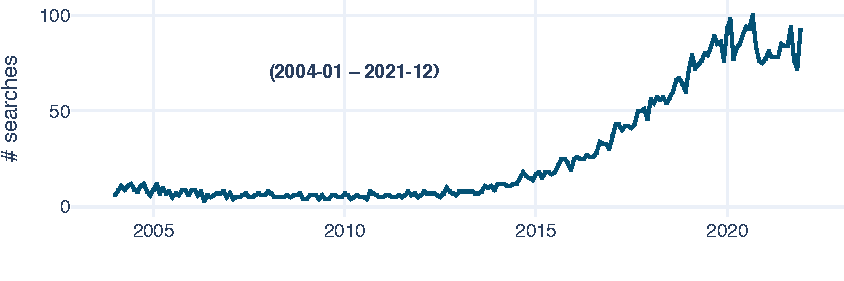
\includegraphics[width=\textwidth]{figures/DataScience/googleTrendsTS.pdf}\label{fig:GoogleTrendsDS:ts}
}

\subfloat[geolocalization]{
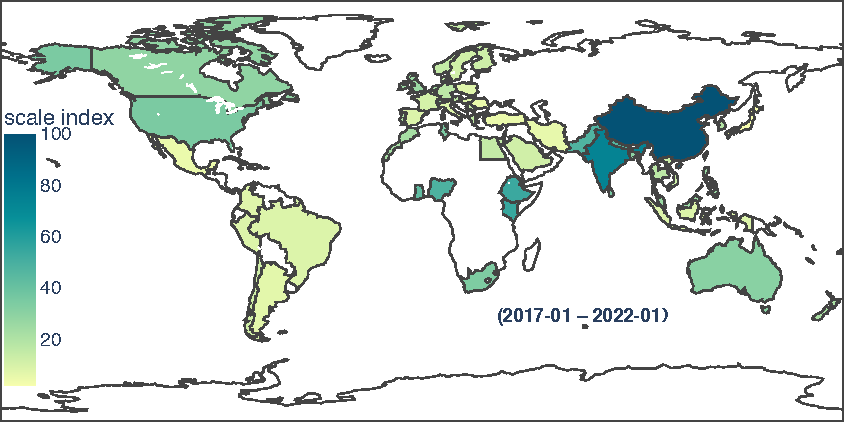
\includegraphics[width=\textwidth]{figures/DataScience/googleTrendsMap.pdf}\label{fig:GoogleTrendsDS:map}
}
\caption{
\textbf{``Data Science" Google searches}. The trend of Google searches for the term ``data science" (\hyperref[fig:GoogleTrendsDS:ts]{a}) and the corresponding geolocalization (\hyperref[fig:GoogleTrendsDS:map]{b}) show an evident increase of the popularity of the subject and its global penetration
} 
\label{fig:GoogleTrendsDS}
\end{figure}
That much so that it was awarded the title of \textquote{sexiest job of the 21st century} \cite{davenport2012sexiest}, and only American universities counted 78 data science programs in 2020 \cite{zhang2021data}.

However, the discussion over data science's essence has a long history, and multiple definitions have been proposed over the years \cite{donoho201750years}.
Although researchers and practitioners are yet to reach a complete agreement on its exact meaning  \cite{ASA2015statement}, \emph{five} common pillars can be identified by the various definitions.
First, \textbf{multidisciplinarity} is indisputably a key element stressed in every definition of data science. 
Second, as the name suggests, the \textbf{focus on data} and adequate techniques to manage and process them is inevitably an essential aspect.
Third, data science requires adopting suitable \textbf{statistical models} to convert data into knowledge.
Fourth, the \textbf{computing infrastructure} that is necessary to manage the data and analyze them efficiently. 
Fifth, a compelling \textbf{visualization and communication} of results that is simple enough to be understood by a heterogeneous and non-technical audience, yet comprehensive of all relevant details to convey valuable insights.

Inspired by these principles, we reckon that the essence of data science ought to be traced back to its practical aspect, which is the starting sparkle and the ultimate destination of any data science investigation.
Indeed, all data science projects share the common target of solving real-life problems in a data-driven fashion.
Although overcoming hampers is not a novel challenge -- in fact, one may see it as a key aspect of the evolution really, which has always been crucial for the progression of species, especially regarding the human kind -- the peculiar feature that distinguishes data science is its framing into a data-oriented paradigm.
Not surprisingly, its explosion comes as a normal response to the increased availability of data we have been experiencing in modern times.
Having data about virtually any aspect of life poses the question of how to leverage this information to tackle unsolved problems and re-think current approaches.
This in turn urges for a methodological framework that provides tools for modeling natural phenomena and learning from their data.
As a consequence, computing infrastructures are needed to manage the data and enable the practical implementation and use of the developed theories.
Hence, the foundational core of data science can be established in the trinomial \textit{\mbox{data-statistics-computing}} that summarizes the practical, theoretical and technical challenges related to the discipline.
\sidenote[Luca][notesyellow]{alternative trinomio: 1) "data-modeling-computing", 2) "data-learning-computing"}
Importantly, the above chain of causes-consequences is not static, as advancements in any of the three areas pave the way for novel research in the others. 
Therefore, each of the components can be seen as both an enabling factor and a stimulus for the others, thus generating a virtuous circle that encourages progress.
% \sidenote[Luca][notesyellow]{Inserire schema circolo virtuoso}
% \sidenote[Luca][notesyellow]{procedere esempi di big data + ML e computing come un enabling factor per la ricerca}
% \note[Luca][notesyellow]{
% The modern popularity of neural networks is a vivid example of how this collaborative interchange acts in practice.
% Born as an altenative way to analyze data \protect \cite{mitchell1989}, they were long time under the radars.
% However, the sudden availability of more data and more powerful computing resources became an enabling factor for their adoption and practical successes.
% This in turn generated the curiosity to test that methodology on a cascade of what-if scenarios:
% bigger datasets, rephrasal of the tasks, ... .
% At the same time, this stimulated a correspondent urge for more efficient and sustainable computing approaches.
% From which it came new computing paradigms (distributed, hadoop, spark, gpu accelerators, ...)
% Which generated new approaches (CV, NLP, ....)

% Which generates the questions on how to collect better data (active learning or CL), and yet more efficient computing solutions (QC).
% This stimulates the question of how to leverage these new solutions, for instance people are studying how to translate classical machine learning building blocks exploiting the computational boost of quantum devices.
% }
Clearly, this process typically requires mixing heterogeneous competencies, from which the necessity for contamination between multiple disciplines contributing to sub-tasks propaedeutic to the final solution.
Also, a clear visualization and communication of the results is paramount to guarantee effective usage of the developed methodologies and avoid misunderstandings in the various inter-domain interactions.
% As a result, a clear visualization and communication is paramount to avoid misunderstandings in the various inter-domain interactions and guarantee effective usage of the developed approaches in practice.
% Guided by the former vision, we frame data science as an applied science that studies how to combine domain expertise with suitable learning approaches and necessary computing resources to process real data for a tangible return.

% Hence, the collection of data and the development of proper methodologies to collect and analyze them justifies the need for statistical theory.
% However, this requires enough computing power to store and process the collected data.
% In turn, the advancement in computer technologies has enabled new paradigms to manage huge amounts of data, and made statistical models feasible, thus also stimulating new research in these fields, that require more computing thus creating a vicious circle that encourage the three discipline to progress.
% Not surprisingly, its explosion comes as a normal response to the increased availability of data about virtually any aspect of life that has led to the so-call big data era.
% Besides that, the progress of computing technologies has been a key enabling factor to allow one one side to store and manage huge amounts of data.
% Also, the enhanced computing power has has made 
% stimulated research on statistical methods to analyze increased quantities of data that could not be possible without sufficient computing power.
% \sidenote[Luca][notesyellow]{Circolo vizioso: menzionare trinomio "data-statistics-computing" e se possibile schema}

% However, the above schema requires complex interaction between different areas, each required profound proficiency to be carried out effectively to produce a valuable result in a timely manner.
% Hence, the need for suitable visualizations that put the last tile to reach valuable insights as a result.
% One of the enabling factors 
% One of these components is surely data. The big data era we are witnessing entails a 
% Also, the increasing availabilty of data about virtually any aspect of life, nowadays allows to tackle problems in a more systematic and critic way, thus the data-driven strategy. 
% Hence, the other pillars come as fundamental 


Guided by the former vision, this work discusses two independent data science projects developed in the scope of multidisciplinary applied research, and describes how the five pillars above are declined for the two use cases.
Despite treating the proposed methodologies in detail, a particular emphasis posits on \textit{i)} the interdisciplinary nature of the projects, \textit{ii)} the origin of the data, the information they carry and the corresponding challenges, and \textit{iii)} the practical impact of our approaches.
Also, specific attention is devoted to data visualization, both in the initial exploration and the presentation of the results, for its crucial role in enabling the communication among experts from various domains.

\subsection*{Structure of the Thesis}

After an initial definition of the discipline of \emph{Data Science}, this thesis is organized as follows.

\Cref{chap:historyDS} draws a historical reconstruction of the evolution of the concept of data science over time, trying to clarify what this subject is all about and set an unambiguous reference framework. 

\Cref{partI} explores in greater detail the work presented in \citeA{morelli2021cresunet}. In particular, \Cref{chap:partI_intro} describes the technique of microscopic fluorescence and its application to life science and biology experiments. The task of counting objects in digital images is then presented, and some relevant literature is reviewed.
\Cref{chap:partI_dataset} describes the \textbf{Fluorescent Neuronal Cells} dataset \cite{clissa2021fluocells}, focusing on data acquisition, data annotations, and peculiar characteristics and challenges. 
In \Cref{chap:partI_methods}, the \textbf{cell ResUnet (c-ResUnet)} \cite{morelli2021cresunet} model is introduced and compared with several alternative architectures. Also, three experimental settings are detailed, which are then used for testing competing architectures through ablation studies.
In \Cref{chap:partI_results}, the performances achieved by the proposed approaches are evaluated both quantitatively and qualitatively.
Finally, \Cref{chap:partI_conclusions} summarizes the main findings of the study and discusses possible extensions.

\Cref{partII} deals with the issue of computing infrastructure management in the context of the Worldwide Large Hadron Collider Computing Grid.
\Cref{ch:opint_intro} introduces the High-Energy Physics community and the related experiments conducted through the Large Hadron Collider (LHC) at the CERN laboratory, with a particular focus on the computing infrastructure adopted for sharing and analyzing the experimental data. 
In particular, \cref{ch:opint} describes more in detail the data flows generated by the LHC and introduces the Operational Intelligence project \cite{opint2020}, a joint effort of different collaborations to automate infrastructure management.
Among its various activities, the subject of troubleshooting transfer failures is taken into account, and some ongoing attempts are outlined alongside our contributions.
\Cref{ch:opint_methods} discusses a possible approach to the problem aimed at supporting current operations by automatically extracting a few error categories (in the order of tens) from the massive amount of daily failed transfers (in the order of millions).
\Cref{ch:opint_results} reports a demonstration of our approach applied to one day of data as a proof of concept for its potential, taking into account both a qualitative interpretation of the results and a quantitative proxy of the performance.
Finally, \cref{ch:opint_conclusions} summarizes the advantages and limitations of the proposed methodology and suggests a possible direction for future developments.

\section{History of Data Science}
\label{chap:historyDS}

The first trace of this debate dates back to \cite{tukey1962future}, where Tukey uses the term \emph{data analysis} to indicate a discipline with the connotations of a \emph{science} and which is \textquote{defined by a ubiquitous problem rather than by a concrete subject}. 
Tukey's description incorporates many aspects seemingly tied closely to applied statistics: 
\begin{displayquote}
procedures for analyzing data, techniques for interpreting the results of such procedures, ways of planning the gathering of data to make its analysis easier, more precise or more accurate, and all the machinery and results of (mathematical) statistics which apply to analyzing data.
\end{displayquote}
Nevertheless, the extent Tukey attributes to data analysis is broader than its philological meaning, as it comprises all of statistics and embeds it in a larger entity \cite{huber2012data, donoho201750years}.
Indeed, Tukey himself sets the boundaries between data analysis and statistics in their respective binding to the strict formalism of mathematics.

In fact, he appeals for a looser attachment to mathematical foundations and suggests focusing on actionable insights rather than theory.
 - scope and usefulness over security
 - inadequate evidence shall suggest right answers
 - maths as judgment rather than proof
 
Finally, Tukey identified four driving forces in the emerging data analysis science:
Four major influences act on data analysis today:
1. The formal theories of statistics
2. Accelerating developments in computers and display devices
3. The challenge, in many fields, of more and ever larger bodies of data
4. The emphasis on quantification in an ever wider variety of disciplines

Despite being released 60 years ago, Tukey's description is incredibly modern and well depicts many activities currently under the umbrella of what we refer to as data science today.
Nonetheless, researchers and practitioners are yet to reach a complete agreement on its definition.

By and large, bla bla bla...
